%!TEX root=../GaugeCNNTheory.tex


\subsection{انتقال موازی بردارهای ویژگی}
\label{sec:transport_local}

کرنل‌های شبکه‌های کانولوشنی ویژگی‌ها را از تمام نقاط $q$ در یک همسایگی اطراف هر نقطه $p$ از منیفولد جمع‌آوری می‌کنند.
از آنجا که ویژگی‌ها در نقاط مختلف در فضاهای بردار ویژگی متفاوتی قرار دارند و نسبت به گیج‌های مختلف بیان می‌شوند، باید قبل از پردازش بیشتر، در امتداد یک مسیر $\gamma$ از $q$ به $p$ \emph{به صورت موازی منتقل} شوند.
ما ابتدا انتقال بردارهای مماس را مورد بحث قرار می‌دهیم، که توسط یک نگاشت انتقال موازی رسمی‌سازی می‌شود:
\begin{align}
	\mathcal{P}_\gamma: \TqM \to \TpM \,.
\end{align}
این انتقال‌دهنده اغلب از اتصال کانونی لوی-چویتا منیفولد محاسبه می‌شود، با این حال، ممکن است در برخی کاربردها مربوط به یک اتصال جایگزین (سازگار با $G$) باشد، همانطور که در ادامه و در مرور ادبیات ما در بخش~\ref{part:literature_review} بیشتر مورد بحث قرار می‌گیرد.
انتقال‌دهنده بردارهای ویژگی (مرتبط با $G$) از انتقال‌دهنده بردارهای مماس تبعیت می‌کند اگر انتقال سازگار با $G$ باشد.


\subsubsection{انتقال‌دهنده‌های بردار مماس}

از نظر آموزشی معقول است که ابتدا با حالت خاص انتقال‌دهنده‌های لوی-چویتا در فضاهای اقلیدسی که در شکل~\ref{fig:transport_flat} به تصویر کشیده شده‌اند، شروع کنیم، قبل از پرداختن به انتقال‌دهنده‌ها و منیفلدهای عمومی‌تر.
در این حالت انتقال موازی مستقل از مسیر انتخاب شده $\gamma$ است و بردار منتقل شده را به معنای معمول در فضاهای اقلیدسی موازی نگه می‌دارد.
توجه داشته باشید که انتقال‌دهنده~$\mathcal{P}_\gamma$ بین فضاهای مماس $\TqM$ و $\TpM$ نگاشت می‌کند و بنابراین مستقل از مختصات است.
با این حال، می‌توان آن را نسبت به مختصات بیان کرد، سپس به جای بردارهای مماس بر روی بردارهای ضریب عددی عمل می‌کند.
شهودی در شکل~\ref{fig:transport_flat} آورده شده است، جایی که چارچوب‌ها در $q$ و $p$ موازی نیستند%
\footnote{
	برخلاف منیفلدهای عمومی، $\R^d$ با مفهوم کانونی موازی بودن چارچوب‌های مرجع همراه است.
}
به طوری که ضرایب $(1,1)^\top$ در $q$ و $\big(\sqrt{2},0\big)^\top$ در $p$ متفاوت هستند، حتی اگر بردارهای مماس (مستقل از مختصات) مربوطه با یکدیگر موازی باشند.
برای دقیق‌تر کردن این موضوع، گیج‌های $\psi_q^{\widetilde{A}}$ و $\psi_p^A$ را در همسایگی‌های $U^{\widetilde{A}}$ از $q$ (قرمز) و $U^A$ از $p$ (سبز) در نظر بگیرید.
فرض کنید یک بردار $v = \big( \psi_q^{\widetilde{A}} \big)^{-1} (v^{\widetilde{A}}) \in \TqM$ با ضرایب $v^{\widetilde{A}} \in \R^d$ داده شده باشد.
ضرایب بردار منتقل شده $\mathcal{P}_\gamma v$ در $p$ سپس توسط:
$
\psi_p^A \circ \mathcal{P}_\gamma (v)
\ =\ \psi_p^A \circ \mathcal{P}_\gamma \circ \big(\psi_q^{\widetilde{A}}\big)^{-1} (v^{\widetilde{A}})
$
داده می‌شود.
نتیجه می‌شود که بیان مختصاتی یک انتقال‌دهنده نسبت به گیج‌های $\widetilde{A}$ و $A$ به صورت زیر است:%
\footnote{
	$g_\gamma^{A\widetilde{A}}$ مقادیری در $\GL{d}$ می‌گیرد اگر ما اتصال‌های دلخواه (با مقدار $\mathfrak{gl}(d)$) و گروه‌های ساختار عمومی $G \leq \GL{d}$ را فرض کنیم.
	برای اتصال لوی-چویتا با مقدار $\mathfrak{so}(d)$ و چارچوب‌های متعامد، یعنی $G=\OO{d}$، ما $g_\gamma^{A\widetilde{A}} \in \OO{d}$ را داریم.
}
\begin{align}\label{eq:transporter_gauge}
	g_\gamma^{A\widetilde{A}} \ :=\ \psi_p^A \circ \mathcal{P}_\gamma \circ \big( \psi_q^{\widetilde{A}} \mkern1mu\big)^{-1} \in\, \GL{d}
\end{align}
عنصر گروهی $g_\gamma^{A\widetilde{A}}$ انتخاب‌های غیرموازی چارچوب‌های مرجع در $q$ و $p$ را در نظر می‌گیرد.
در $\R^d$، معمولاً فرض می‌شود که تمام چارچوب‌ها موازی هستند به طوری که تمام مختصات‌بندی‌های انتقال‌دهنده‌های لوی-چویتا بدیهی می‌شوند.%
\footnote{
	\CNN{}های سنتی در $\R^d$ به طور ضمنی این فرض را از چارچوب‌های موازی (شکل~\ref{fig:G_structure_intro_a}) و انتقال‌دهنده‌های بدیهی می‌کنند.
}

\begin{figure*}
	\centering
	\begin{subfigure}[b]{0.5\textwidth}
		\centering
		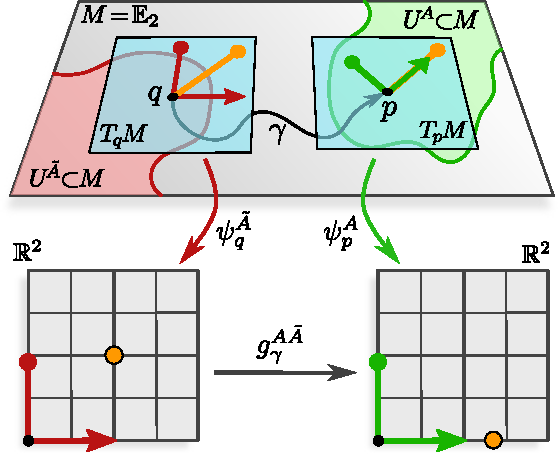
\includegraphics[width=.95\textwidth]{figures/transport_flat.pdf}
		\vspace*{1ex}
		\caption{\small
			انتقال موازی و مختصات‌بندی آن در یک فضای مسطح.
		}
		\label{fig:transport_flat}
	\end{subfigure}
	\hfill
	\begin{subfigure}[b]{0.4\textwidth}
		\centering
		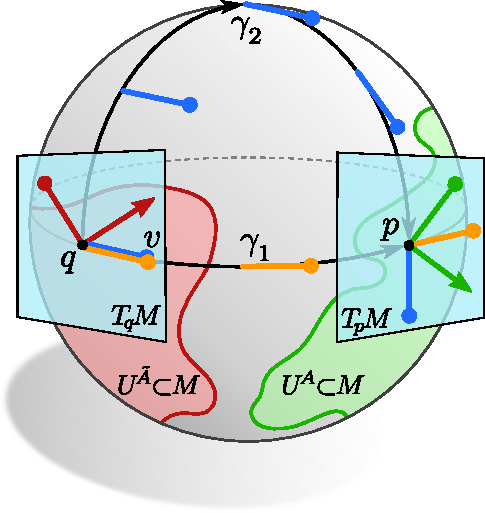
\includegraphics[width=\textwidth]{figures/transport_sphere.pdf}
		\vspace*{-2ex}
		\caption{\small
			انتقال موازی در کره $S^2$.
		}
		\label{fig:transport_sphere}
	\end{subfigure}
	\caption{\small
		انتقال موازی بردارهای مماس $v\in \TqM$ در $q$ به $\mathcal{P}_\gamma v \in \TpM$ در $p$.
		شکل~\ref{fig:transport_flat} حالت خاص انتقال‌دهنده‌های لوی-چویتا را در فضاهای اقلیدسی مسطح $M = \Euc_d$ بصری‌سازی می‌کند.
		مستقل از مسیر انتخاب شده $\gamma$, انتقال لوی-چویتا بردار (نارنجی) را به معنای معمول در فضاهای اقلیدسی موازی نگه می‌دارد.
		گیج‌های $\psi_q^{\widetilde{A}}$ (قرمز) و $\psi_p^A$ (سبز) امکان بیان انتقال‌دهنده مستقل از مختصات را توسط یک عنصر گروهی
		$g_\gamma^{A\widetilde{A}} = \psi_p^A \circ \mathcal{P}_\gamma \circ \big(\psi_q^{\widetilde{A}}\big)^{-1} \in \GL{d}$
		فراهم می‌کنند که تغییر ضرایب بردار را در نظر می‌گیرد اگر چارچوب هدف با چارچوب منبع منتقل شده مطابقت نداشته باشد.
		شکل~\ref{fig:transport_sphere} انتقال لوی-چویتا را در ۲-کره~$S^2$ نشان می‌دهد، مقایسه کنید با~معادله~\eqref{eq:sphere_transport_embedded}.
		انتقال‌دهنده‌های $\mathcal{P}_{\mkern-2mu\gamma_1}$ و $\mathcal{P}_{\mkern-2mu\gamma_2}$ در امتداد مسیرهای مختلف $\gamma_1$ و $\gamma_2$ به طور کلی با یکدیگر اختلاف دارند.
		همانند فضاهای مسطح، انتقال‌دهنده‌های مستقل از مختصات را می‌توان توسط عناصر گروهی که بر روی ضرایب نسبت به چارچوب‌های مختصاتی در $q$ و $p$ عمل می‌کنند، بیان کرد.
	}
	\label{fig:transport}
\end{figure*}


از آنجا که انتقال‌دهنده در معادله~\eqref{eq:transporter_gauge} وابسته به مختصات است، ما علاقه‌مند به تبدیل‌های گیج آن هستیم.
گیج‌های $\psi_q^{\widetilde{B}}$ و $\psi_p^B$ را دو گیج جایگزین در همسایگی‌های $q$ و $p$ در نظر بگیرید.
از نمودار جابجایی:
\begin{equation}\label{cd:transporter_trivialization}
	\begin{tikzcd}[column sep=50pt, row sep=25pt, font=\normalsize]
		\R^d
		\arrow[dd, "g_q^{\widetilde{B}\widetilde{A}}\cdot\ "']
		\arrow[rrr, "g_\gamma^{A\widetilde{A}}\cdot"]
		& &[-1ex] &
		\R^d
		\arrow[dd, "\ g_p^{BA}\cdot"]
		\\
		&
		\TqM
		\arrow[ul, "\psi_q^{\widetilde{A}}"]
		\arrow[dl, "\psi_q^{\widetilde{B}}"']
		\arrow[r, "\mathcal{P}_\gamma"]
		&
		\TpM
		\arrow[ur, "\psi_p^A"']
		\arrow[dr, "\psi_p^B"]
		\\
		\R^d
		\arrow[rrr, "g_\gamma^{B\widetilde{B}}\cdot"']
		& & &
		\R^d
	\end{tikzcd}
\end{equation}
می‌توان خواند که انتقال‌دهنده‌ها در گیج‌های مختلف توسط:
\begin{align}\label{eq:transporter_gauge_trafo}
	g_\gamma^{B\widetilde{B}}
	\ =\ g_p^{BA}\, g_\gamma^{A\widetilde{A}}\, \big(g_q^{\widetilde{B}\widetilde{A}} \mkern1mu\big)^{-1}
\end{align}
مرتبط هستند.
توجه داشته باشید که شباهت این قانون تبدیل و نمودار جابجایی به آنچه در معادلات~\eqref{eq:matrix_gaugetrafo} و~\eqref{eq:linear_map_TpM_diagram} آمده است.
تفاوت بین هر دو این است که انتقال‌دهنده دارای دامنه $\TqM$ و دامنه مشترک $\TpM$ متفاوتی است که توسط گیج‌های مختلف و مستقل از یکدیگر تسهیم شده‌اند و بنابراین به طور مستقل تبدیل می‌شوند.


به طور کلی، انتقال موازی بردارهای مماس توسط یک انتخاب اتصال تعیین می‌شود، به عنوان مثال (اما نه لزوماً) توسط اتصال کانونی لوی-چویتا یک منیفولد ریمانی.
یک اتصال را می‌توان به عنوان مجموعه‌ای از انتقال‌دهنده‌های بی‌نهایت کوچک بین فضاهای مماس مجاور در نظر گرفت، به طوری که انتقال‌دهنده کامل $\mathcal{P}_\gamma$ با انتگرال‌گیری اتصال در امتداد مسیر $\gamma$ به دست می‌آید.
انتقال‌دهنده‌ها در امتداد مسیرهای مختلف $\gamma_1$ و~$\gamma_2$ از $q$ به~$p$ نیازی به مطابقت ندارند، که در شکل~\ref{fig:transport_sphere} با انتقال‌دهنده‌های لوی-چویتا در 2-کره~$S^2$ مثال زده شده است، مقایسه کنید با~معادله~\eqref{eq:sphere_transport_embedded}.
همانند فضاهای مسطح، انتقال‌دهنده‌های مستقل از مختصات را می‌توان توسط معادله~\eqref{eq:transporter_gauge} نسبت به گیج‌ها بیان کرد.
تبدیل‌های گیج چنین انتقال‌دهنده‌های مختصات‌بندی شده دوباره توسط معادله~\eqref{eq:transporter_gauge_trafo} داده می‌شوند.
انتقال‌دهنده‌ها در یک منیفولد داده شده می‌توانند در اصل به صورت تحلیلی از اتصال محاسبه شوند \cite{gallier2019diffgeom1,nakahara2003geometry} و گاهی اوقات می‌توانند به صورت فرم بسته بیان شوند، به عنوان مثال برای کره $S^2$، معادله~\eqref{eq:sphere_transport_embedded}.
چندین الگوریتم عددی برای محاسبه انتقال‌دهنده‌های موازی در مش‌ها وجود دارد؛ به بخش~\ref{sec:surfaces_geom_mesh} مراجعه کنید.
ما به جزئیات بیشتر در مورد نحوه محاسبه انتقال‌دهنده‌های بردار مماس $\mathcal{P}_\gamma$ نخواهیم پرداخت بلکه به سادگی آن‌ها را داده شده فرض می‌کنیم.


\subsubsection{انتقال‌دهنده‌های بردار ویژگی}

معادله~\eqref{eq:gauge_trafo_features} قانون تبدیل ضرایب بردار ویژگی را توسط \emph{نوع میدان} آن‌ها ($\rho$) تعریف می‌کند.
انتقال‌دهنده موازی آن‌ها، که نسبت به گیج‌های $\psi_q^{\widetilde{A}}$ و $\psi_p^A$ بیان می‌شود، به طور مشابه با پیچیدن انتقال‌دهنده ضریب بردار مماس در این نمایش میدان داده می‌شود، یعنی توسط:
\begin{align}
	\rho\big( g_\gamma^{A\widetilde{A}} \big) \,.
\end{align}
توجه داشته باشید که -- از آنجا که $\rho:G\to\GL{c}$ یک نمایش $G$ است ـ این ساختار تنها زمانی به خوبی تعریف می‌شود که تمام انتقال‌دهنده‌ها~$g_\gamma^{A\widetilde{A}}$ (برای مسیرهای دلخواه $\gamma$ و چارچوب‌های $A$، $\widetilde{A}$) واقعاً مقادیری در گروه ساختار انتخاب شده~$G$ بگیرند.
اینکه آیا این حالت صادق است یا خیر هم به انتخاب خاص $G$-ساختار (یا $G$-اطلس) و هم به انتقال‌دهنده‌ها (یا اتصال) مورد نظر بستگی دارد ـ آن‌ها باید \emph{سازگار} باشند \cite{wendlLectureNotesBundles2008}.


تمام شبکه‌های کانولوشنی (بنابراین انتقال می‌دهند) بردارهای ویژگی را به نحوی جمع‌آوری می‌کنند، و بنابراین برخی انتخاب از اتصال و $G$-ساختار را فرض می‌کنند.
اگر $G$-ساختار انتخاب شده با اتصال لوی-چویتا ناسازگار باشد، این به معنای آن است که این مدل‌ها -- اغلب به طور ضمنی ـ یک اتصال جایگزین و سازگار با $G$ را برای جمع‌آوری ویژگی‌ها فرض می‌کنند.
خواننده فعلاً نباید نگران انتخاب‌های خاص اتصال‌ها باشد، که در مرور ادبیات ما در بخش~\ref{part:literature_review} روشن‌تر خواهد شد.
در ادامه این بخش، ما بیشتر در مورد سازگاری $G$ اتصال‌ها و $G$-ساختارها توضیح خواهیم داد.
با فرض اینکه \emph{انتقال‌دهنده‌های ویژگی در ادامه همیشه به خوبی تعریف خواهند شد}، این بخش را می‌توان با خیال راحت در اولین مطالعه نادیده گرفت.

بحث دقیق‌تر و مستقل از مختصات انتقال‌دهنده‌ها در بندل‌های بردار ویژگی مرتبط را می‌توان در بخش~\ref{sec:bundle_transport} یافت.


\subsubsection{سازگاری اتصال‌ها و \textit{$G$}-ساختارها}

یک اتصال با یک $G$-ساختار $\GM$ \emph{سازگار با $G$} نامیده می‌شود اگر عبارات مختصاتی $g_\gamma^{A\widetilde{A}}$ انتقال‌دهنده‌های $\mathcal{P}_\gamma$ آن نسبت به هر چارچوب $A$، $\widetilde{A}$ از $\GM$ مقادیری در گروه ساختار~$G$ بگیرند \cite{wendlLectureNotesBundles2008}.%
\footnote{
	به طور معادل، \emph{فرم ۱-اتصال} اتصال، که نسبت به چارچوب‌های $\GM$ بیان می‌شود، ملزم به داشتن مقدار $\mathfrak{g}$ است، که در آن $\mathfrak{g}$ نشان‌دهنده جبر لی~$G$ است.
	به طور انتزاعی‌تر، ما به \emph{اتصال‌های اصلی اهرسمن} در بندل اصلی $G$ ($\GM$) علاقه‌مندیم.
}
یک اتصال سازگار با $G$ منجر به انتقال‌دهنده‌های بردارهای ویژگی مرتبط با $G$ می‌شود.

برای روشن کردن این شرط سازگاری تا حدی انتزاعی، چند مثال خاص را مورد بحث قرار می‌دهیم.
یک مثال ساده، اتصال لوی-چویتا در $\R^2$ است، شکل~\ref{fig:transport_flat}.
دو ساختار $\{e\}$ در $\R^2$ که در اشکال~\ref{fig:frame_field_automorphism_1} و~\ref{fig:frame_field_automorphism_2} نشان داده شده‌اند را در نظر بگیرید.
در اینجا $G=\{e\}$ است، به این معنی که نوع میدان $\rho: \{e\} \to \GL{c}$ یک نمایش $\{e\}$ است، به طوری که انتقال موازی بردارهای ویژگی تنها در صورتی می‌تواند تعریف شود که عبارات مختصاتی $g_\gamma^{A\widetilde{A}}$ مقادیری در~$\{e\}$ بگیرند، یعنی بدیهی باشند.
از آنجا که ساختار $\{e\}$ در شکل~\ref{fig:frame_field_automorphism_1} از چارچوب‌های "موازی" تشکیل شده است، این امر واقعاً همینطور است ـ بنابراین اتصال لوی-چویتا با این ساختار $\{e\}$ سازگار است.
در مقابل، چارچوب‌های ساختار $\{e\}$ در شکل~\ref{fig:frame_field_automorphism_2} نسبت به یکدیگر "چرخانده شده‌اند"، که منجر به عبارات مختصاتی غیربدیهی $g_\gamma^{A\widetilde{A}}$ می‌شود که مقادیری در $\SO{2}$ می‌گیرند (در شکل~\ref{fig:transport_flat} بصری‌سازی شده است).
از آنجا که نوع میدان $\rho: \{e\} \to \GL{c}$ چرخش‌ها را مدیریت نمی‌کند، امکان تعریف انتقال لوی-چویتا ویژگی‌های مرتبط با این ساختار $\{e\}$ وجود ندارد ـ آن‌ها ناسازگار هستند.
به عنوان مثال دوم، اتصال لوی-چویتا در $S^2$ را در نظر بگیرید، که در شکل~\ref{fig:transport_sphere} نشان داده شده است.
انتقال در این حالت همیشه وابسته به مسیر خواهد بود و منجر به بردارهای چرخانده شده متفاوت خواهد شد، که دلالت دارد بر اینکه $g_\gamma^{A\widetilde{A}}$ مقادیری در $\SO{2}$ خواهد گرفت.
بردارهای ویژگی که باید مطابق با اتصال لوی-چویتا منتقل شوند، بنابراین باید از نوع $\rho: \SO{2} \to \GL{c}$ باشند که یک نمایش $\SO{2}$ است.
این امر حداقل نیازمند ساختار $\SO{2}$ در $S^2$ است که در شکل~\ref{fig:G_structure_S2_1} نشان داده شده است.
ساختار $\{e\}$ در $S^2$ از شکل~\ref{fig:G_structure_S2_2} با اتصال لوی-چویتا ناسازگار است.


از آنجا که اتصال لوی-چویتا یک اتصال متریک است، طول و زاویه بین بردارهای مماس را حفظ می‌کند، و بنابراین چارچوب‌های متعامد را به چارچوب‌های متعامد منتقل می‌کند.
نتیجه می‌شود که اتصال لوی-چویتا \emph{همیشه} با ساختار $\OO{d}$ چارچوب‌های متعامد سازگار است، که نسبت به آن $g_\gamma^{A\widetilde{A}}$ مقادیری در~$\OO{d}$ می‌گیرد.
اگر منیفولد قابل جهت‌گیری باشد، دست‌سانی چارچوب توسط انتقال‌دهنده‌های لوی-چویتا حفظ می‌شود، به این معنی که آن‌ها تضمین شده‌اند که با ساختارهای $\SO{d}$ چارچوب‌های متعامد راست‌گرد در~$M$ سازگار باشند.
تمام شبکه‌های کانولوشنی در مرور ادبیات ما در بخش~\ref{part:literature_review} که بر اساس ساختارهای $\SO{d}$ هستند، ویژگی‌ها را از طریق انتقال‌دهنده‌های لوی-چویتا جمع‌آوری می‌کنند.


اگر یک $G$-ساختار داده شده با اتصال لوی-چویتا ناسازگار باشد، باید یک اتصال جایگزین و سازگار با $G$ را برای انتقال بردارهای ویژگی تعریف کرد.
برجسته‌ترین مثال در مرور ادبیات ما، \emph{اتصال‌های بدیهی} در ساختارهای $\{e\}$ است.
یک اتصال بدیهی با خاصیت \emph{مستقل از مسیر} بودن انتقال آن مشخص می‌شود \cite{craneTrivialConnectionsDiscrete2010}.
هر ساختار $\{e\}$ یک اتصال بدیهی منحصر به فرد را نتیجه می‌دهد، که بردارهای مماس را به گونه‌ای منتقل می‌کند که زاویه یکسانی را با چارچوب‌های مرجع ساختار $\{e\}$ حفظ کنند.
این امر دلالت دارد بر اینکه $g_\gamma^{A\widetilde{A}} = e$, یعنی آن‌ها بردارهای ضریب را در $\R^c$ (نسبت به چارچوب‌های ساختار $\{e\}$) بدون تغییر مقادیر عددی آن‌ها منتقل می‌کنند.
چنین انتقال‌دهنده‌هایی در شبکه‌های کانولوشنی استفاده می‌شوند که انتقال‌دهنده‌های غیربدیهی را به صراحت مدل نمی‌کنند ـ که در مورد \emph{تمام} شبکه‌های دارای $G=\{e\}$ در جدول~\ref{tab:network_instantiations} صادق است، به ویژه آن‌هایی که در بخش‌های~\ref{sec:spherical_CNNs_azimuthal_equivariant} و~\ref{sec:e_surface_conv} هستند.
توجه داشته باشید که اتصال بدیهی تنها اتصالی است که با یک ساختار $\{e\}$ سازگار است.

همانطور که در بالا ذکر شد، \emph{هر} شبکه کانولوشنی برخی انتخاب از $G$-ساختار و اتصال سازگار را فرض می‌کند،
اغلب اتصال‌های لوی-چویتا یا اتصال‌های بدیهی.

بخش~\ref{sec:bundle_transport} به طور مفصل در مورد سازگاری انتقال‌دهنده‌ها و $G$-ساختارها از دیدگاه مستقل از مختصات توضیح می‌دهد.